\chapter{リウヴィルの定理とハミルトン流}

\lectureoverview{ハミルトンの方程式は運動方程式を単に書き換える以上のことをする。それらは相空間上の速度場を定義し、その発散はゼロである。この単純な相殺がリウヴィルの定理である。すなわち、ハミルトン的発展は相空間の体積を保存する。その意味が見えてくる順序でこれに到達しよう---まずエネルギー保存、次に等エネルギー面、次に可能な初期条件の流体、そして最後に体積保存流と散逸的吸い込みの対比である。同じ言語が自然にポアソン括弧へと導く。}

\section{なぜもう一つの力学の形式なのか}

我々が求める定理は、講義の冒頭で導入した可逆な状態図の連続的古典対応物である。可逆な離散法則では、各状態には入る矢印が一つと出る矢印が一つある。現在は次の状態と前の状態の両方を決定するのに十分である。悪い法則は多くの状態を一つの吸い込みへ送る。未来は決定されても、過去はもはや回復できない。

リウヴィルの定理は、状態の集合が連続的な相空間であるとき、その区別がどうなるかを述べる。一つの矢印が入り一つの矢印が出るを置き換える表現は\emph{入る流れと同じだけ出る流れ}である。しかしその表現を数学的にする前に、ハミルトンの方程式から流れを再構成する必要がある。

そうすることには歴史的な謎がある。ハミルトン、ヤコビ、ラグランジュ、ポアソンは、それらの形式が不可欠となる量子論を知らずに、精巧で美しい古典力学の形式を築いた。ニュートンには直接の目標があった。惑星運動である。ラグランジュとハミルトンも目の前に物理的問題を持っていたが、彼らは一つの軌道をはるかに超えた類似と構造を追求した。力学における停留作用は光学における最小時間原理に似ていた。光線の運動と粒子の運動は平行な数学的形式に置くことができた。構造自体が物理学を含んでいるように見えたので、彼らは方程式を単純化し、並べ替え、統一した。

我々は今、この直感が並外れて生産的であったことを知っている。論理的には、古典力学の多くの特徴は量子力学の極限として理解できる。歴史的には順序は逆であった。古典的構造が先に見つかり、そのより深い用途が明らかになったのはずっと後である。ファインマンに帰される挑発的な冗談は、内部で追求される数学と、外部のパートナーである物理世界によって制約される物理学を対比することでその点を示した。その冗談は論証ではないが、この区別は有用である。自然がこれらの形式的構造を繰り返し選ぶので、ここでは形式的な美しさが重要なのである。

\begin{classroomqa}
  \audiencequestion{ニュートンは運動エネルギーの現代的概念を持っていたか、そしてエネルギーの概念はどこから始まったのか。
  \lecturetimestamp{00:04:24--00:05:50}}
  \lecturerresponse{ニュートンの力学は力と運動を中心に組織されており、成熟した一般的エネルギー原理を中心にしていたわけではない。正確な歴史的優先順位は議論では決着していない。ライプニッツの\emph{vis viva}、\(\sum_i m_i v_i^2\)は重要な前身であり、現代の運動エネルギーの二倍に等しい。後の熱に関する研究が熱と力学的仕事の間の変換を中心にした。初期の熱素説は熱を保存される実体として扱ったので、交換可能なエネルギー形態という現代の考えは徐々にしか現れなかった。}
\end{classroomqa}

\section{ハミルトンの方程式とエネルギー保存}

系が\(n\)個の正準対を持つとしよう、
\begin{equation}
  (q_i,p_i),\qquad i=1,\ldots,n.
  \label{eq:l7-canonical-pairs}
\end{equation}
各座標に対して一つの運動量があり、各運動量に対して一つの座標がある。運動法則は一つの関数にまとめられる、
\begin{equation}
  H=H(q_1,\ldots,q_n,p_1,\ldots,p_n,t),
  \label{eq:l7-hamiltonian}
\end{equation}
そしてハミルトンの方程式は
\begin{equation}
  \boxed{
  \dot q_i=\frac{\partial H}{\partial p_i},
  \qquad
  \dot p_i=-\frac{\partial H}{\partial q_i}.}
  \label{eq:l7-hamilton-equations}
\end{equation}
符号は正準構造の一部である。\(q\)方程式はプラス符号を持ち、\(p\)方程式はマイナス符号を持つ。

\begin{figure}[htbp]
  \centering
  \includegraphics[width=0.82\textwidth]{lecture_07_figure_02.png}
  \caption{正準変数、関数\(H(q,p)\)、およびまとめの冒頭にある運動量側のハミルトン方程式。}
  \lectureframe{00:07:29}
\end{figure}

方程式は添字付きの対で来るが、力学が対ごとに分離する必要はない。ハミルトニアンはすべての\(q_i\)と\(p_i\)を結合しうるので、例えば\(\dot p_1\)は系全体の状態に依存しうる。

\begin{classroomqa}
  \audiencequestion{この提示は今や公理的か。\(p\)と\(q\)の間にはどのような関係が仮定されているか。
  \lecturetimestamp{00:17:08--00:18:18}}
  \lecturerresponse{ハミルトンの方程式は、\(H(q,p)\)と正準対が指定されれば、形式的理論を定義する。普遍的な追加仮定\(p=m\dot q\)は存在しない。その関係は、二次の運動エネルギーをもつ通常のデカルト粒子に対して成り立つが、他の座標や他のハミルトニアンは他の運動量--速度関係を与える。方程式自体が\(\dot q_i=\partial H/\partial p_i\)を通じてその関係を与える。提案されたハミルトニアンが自然界で実現されているかどうかは、さらなる物理的問題である。}
\end{classroomqa}

これでエネルギー保存を一行の推論で回復できる。軌道に沿って、\(H\)の全微分は
\begin{equation}
  \frac{dH}{dt}
  =
  \sum_i\left(
    \frac{\partial H}{\partial q_i}\dot q_i
    +\frac{\partial H}{\partial p_i}\dot p_i
  \right)
  +\frac{\partial H}{\partial t}.
  \label{eq:l7-total-h-derivative}
\end{equation}
最後の項は、おそらく外部から指定されたパラメータが変化しているために、\(q\)と\(p\)を固定したときの明示的な時間依存性を意味する。式~\eqref{eq:l7-hamilton-equations}を代入すると、
\begin{align}
  \frac{dH}{dt}
  &=
  \sum_i\left[
    \frac{\partial H}{\partial q_i}
    \frac{\partial H}{\partial p_i}
    -\frac{\partial H}{\partial p_i}
    \frac{\partial H}{\partial q_i}
  \right]
  +\frac{\partial H}{\partial t}\\
  &=\frac{\partial H}{\partial t}.
  \label{eq:l7-h-energy-rate}
\end{align}
和の中の各項はその相棒と相殺する。したがって、
\begin{equation}
  \frac{\partial H}{\partial t}=0
  \quad\Longrightarrow\quad
  \frac{dH}{dt}=0.
  \label{eq:l7-energy-conservation}
\end{equation}
閉じた、時間並進不変な系では、ハミルトニアンは保存され、エネルギーである。

\begin{classroomqa}
  \audiencequestion{ハミルトニアンが時間に明示的に依存する場合、何が変わるか。\lecturetimestamp{00:10:32--00:12:33}}
  \lecturerresponse{その場合、式~\eqref{eq:l7-h-energy-rate}は依然として成り立つが、部分系のエネルギーは一定である必要はない。明示的な時間依存性は通常、系とエネルギーを交換する省略された駆動源を表す。その駆動源がより大きな閉じた系の力学的部分に昇格されれば、より大きなハミルトニアンは再び時間独立となり、その全エネルギーは保存される。}
\end{classroomqa}

\section{相空間における幾何学としてのエネルギー}

ここで\(H\)が明示的な時間依存性をもたないと仮定する。初期条件は数\(E\)を固定し、位相点は
\begin{equation}
  H(q,p)=E.
  \label{eq:l7-energy-surface}
\end{equation}
上にとどまる。相空間は\(2n\)次元をもつ。正則点では、その座標間の一つの方程式が\((2n-1)\)次元超曲面を定義する。\(E\)の異なる値は異なる超曲面を与える。それらは閉じている必要もコンパクトである必要もない。エネルギー保存が言うのは、それらの一つから始まった軌道がそれを決して離れないということだけである。

前回の講義の適応された調和振動子に対して、
\begin{equation}
  H=\frac{\omega}{2}(p^2+q^2).
  \label{eq:l7-oscillator-hamiltonian}
\end{equation}
したがって各定エネルギー集合は円であり、
\begin{equation}
  p^2+q^2=\frac{2E}{\omega}.
  \label{eq:l7-oscillator-circle}
\end{equation}

\begin{figure}[htbp]
  \centering
  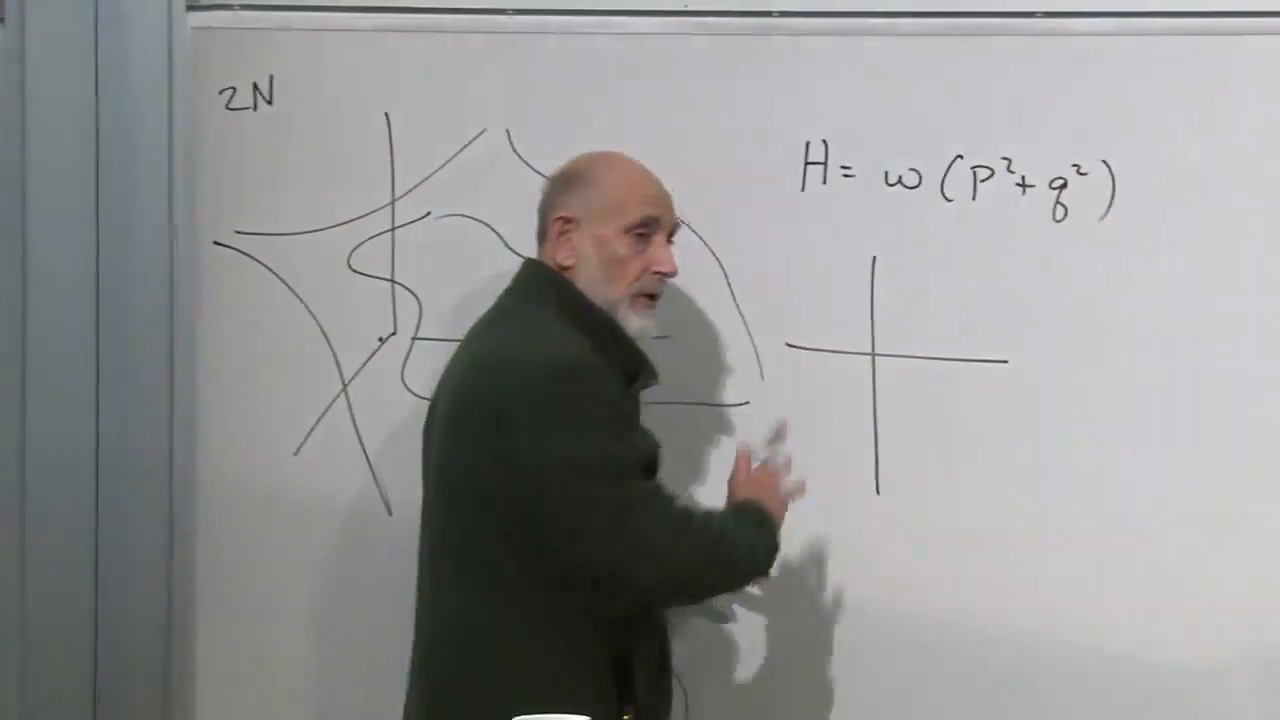
\includegraphics[width=0.84\textwidth]{lecture_07_figure_04.png}
  \caption{定エネルギー面を導入するために用いられた\(2n\)次元相空間のスケッチと調和振動子ハミルトニアン。}
  \lectureframe{00:15:20}
\end{figure}

運動方程式、
\begin{equation}
  \dot q=\omega p,\qquad \dot p=-\omega q,
  \label{eq:l7-oscillator-flow}
\end{equation}
は点をその円の周りで時計回りに動かす。エネルギー方程式はどの曲線が運動を含むかを教え、ハミルトンの方程式はその曲線に沿った方向と速さを教える。

\begin{figure}[htbp]
  \centering
  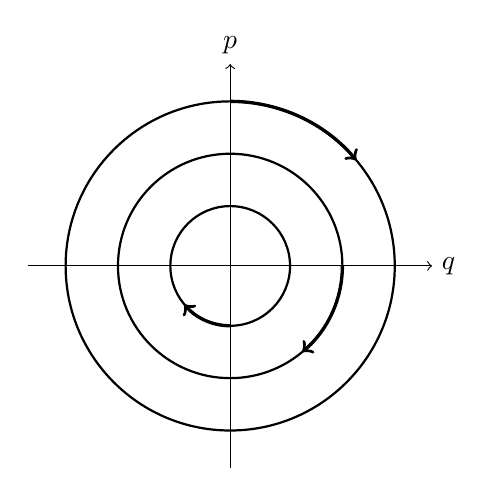
\begin{tikzpicture}[scale=0.95]
    \draw[->] (-2.7,0) -- (2.7,0) node[right] {\(q\)};
    \draw[->] (0,-2.7) -- (0,2.7) node[above] {\(p\)};
    \draw[thick] (0,0) circle (0.8);
    \draw[thick] (0,0) circle (1.5);
    \draw[thick] (0,0) circle (2.2);
    \draw[->,very thick] (0,2.2) arc[start angle=90,end angle=40,radius=2.2];
    \draw[->,very thick] (1.5,0) arc[start angle=0,end angle=-50,radius=1.5];
    \draw[->,very thick] (0,-0.8) arc[start angle=-90,end angle=-140,radius=0.8];
  \end{tikzpicture}
  \caption{一定エネルギーが円を与え、振動子方程式が時計回りの接ベクトル流を与える。}
\end{figure}

\begin{classroomqa}
  \audiencequestion{ハミルトンの二つの方程式と\(H=E\)は同じ方程式のいくつかの版か。
  \lecturetimestamp{00:15:53--00:17:06}}
  \lecturerresponse{いいえ。ハミルトンの方程式は一つの正準対に対する二つの一階の運動法則である。それらは\(dH/dt=0\)を導き、そこから\(H=E\)が従う。\(E\)の値は初期条件によって選ばれる。方程式\(H=E\)は曲面を同定するが、それ自体ではその曲面上の速度を指定しない。}
\end{classroomqa}

\section{一つの状態から状態の流れへ}

一つの初期条件を追う代わりに、相空間にあらゆる可能な初期条件を撒き散らし、時計を始める。各点は完全な可能な状態であり、各状態はハミルトンの方程式に従って動く。この撒き散らしは塵または想像上の流体として想像できる。相空間に物質的なものは何も注がれていない。流体はすべての軌道を一度に見るための方法である。

相空間の速度場は
\begin{equation}
  \mathbf V(q,p,t)
  =
  (\dot q_1,\ldots,\dot q_n,\dot p_1,\ldots,\dot p_n).
  \label{eq:l7-phase-velocity}
\end{equation}
一つの正準対に対しては
\begin{equation}
  V_q=\dot q=\frac{\partial H}{\partial p},
  \qquad
  V_p=\dot p=-\frac{\partial H}{\partial q}.
  \label{eq:l7-phase-components}
\end{equation}
と書く。各点でハミルトニアンは、位相点が次にどこへ行くべきかを告げるベクトルを割り当てる。\(H\)が時間独立なら、ベクトル場は定常である。同じ位相点に戻れば同じ速度が得られる。\(H\)が時間に依存するなら、ベクトル場自体が時間とともに変化するが、それでも各瞬間に定義されている。

\begin{figure}[htbp]
  \centering
  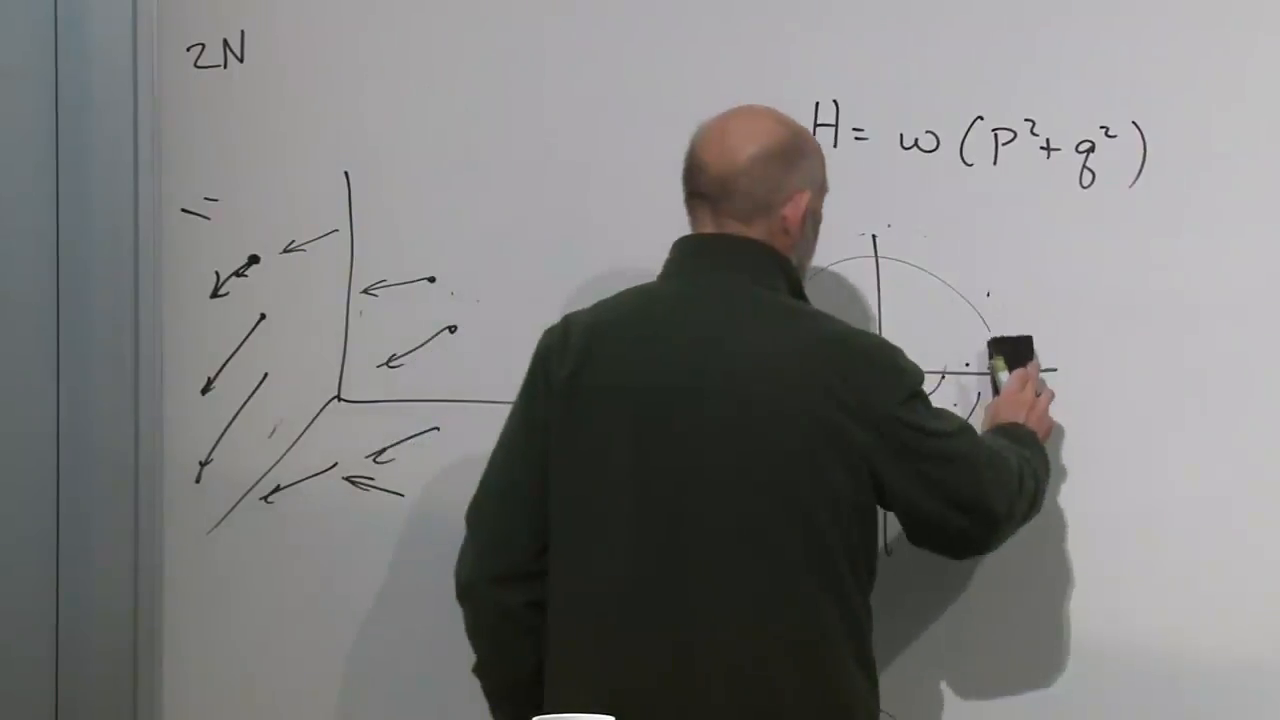
\includegraphics[width=0.84\textwidth]{lecture_07_figure_05.png}
  \caption{調和振動子の速度場。ベクトルは円に接し、原点に向かって短くなる。}
  \lectureframe{00:24:50}
\end{figure}

調和振動子では、すべての半径が角速度\(\omega\)で回転する。原点近くの点は、同じ周期でより短い円を進むため、より小さな線速度をもつ。したがって塵全体は剛体の回転木馬のように回転する。

\begin{classroomqa}
  \audiencequestion{剛体回転とは、すべての振動子の軌道が同じ周期をもつという意味か。\lecturetimestamp{00:21:10--00:21:42}}
  \lecturerresponse{はい。その振幅依存性のなさが調和振動子を特徴づける特別な性質である。小さな円では位相空間速度の大きさがより小さいにもかかわらず、どの円も同じ角振動数\(\omega\)でたどられる。}
\end{classroomqa}

\begin{classroomqa}
  \audiencequestion{位相空間速度はどの点でも同じか。\lecturetimestamp{00:24:29--00:25:37}}
  \lecturerresponse{いいえ。その向きも大きさも一般には位置によって変わる。振動子の場合、ベクトルはその地点の円に接し、大きさは\(\omega\sqrt{p^2+q^2}\)である。ベクトル場とは各点に一つのベクトルが割り当てられたものを意味し、同一のベクトルがどこにでも複製されているのではない。}
\end{classroomqa}

\begin{classroomqa}
  \audiencequestion{この想像上の流体の粒子と密度とは、正確には何か。\lecturetimestamp{00:56:03--00:58:40}}
  \lecturerresponse{各点は、力学系全体のある一つの完全な状態である。一つの物理的粒子ではない。一次元空間を運動する五つの粒子には五つの位置と五つの運動量が必要であり、したがって十次元の位相空間を要する。三次元では三十次元を要する。この塵は代替的な状態の集まりである。流体の描像が気を散らすなら、初期条件のある領域を取り、その中の各点を時間発展させ、その前後で位相空間体積を比較すればよい。}
\end{classroomqa}

\section{圧縮と発散}

この想像上の流体が体積を失うかどうかを問うために、まず一次元から始める。直線上の点が速度\(v(x)\)で運動するとする。\(\delta x\)だけ離れた二つの近い点の速度差は
\begin{equation}
  \delta v \simeq \frac{dv}{dx}\,\delta x.
  \label{eq:l7-one-dimensional-strain}
\end{equation}
である。\(dv/dx>0\)なら前方の点がより速く動き、間隔は伸びる。\(dv/dx<0\)なら圧縮される。したがって定常な一次元非圧縮流は
\begin{equation}
  \frac{dv}{dx}=0.
  \label{eq:l7-one-dimensional-incompressible}
\end{equation}
を満たす。

\begin{figure}[htbp]
  \centering
  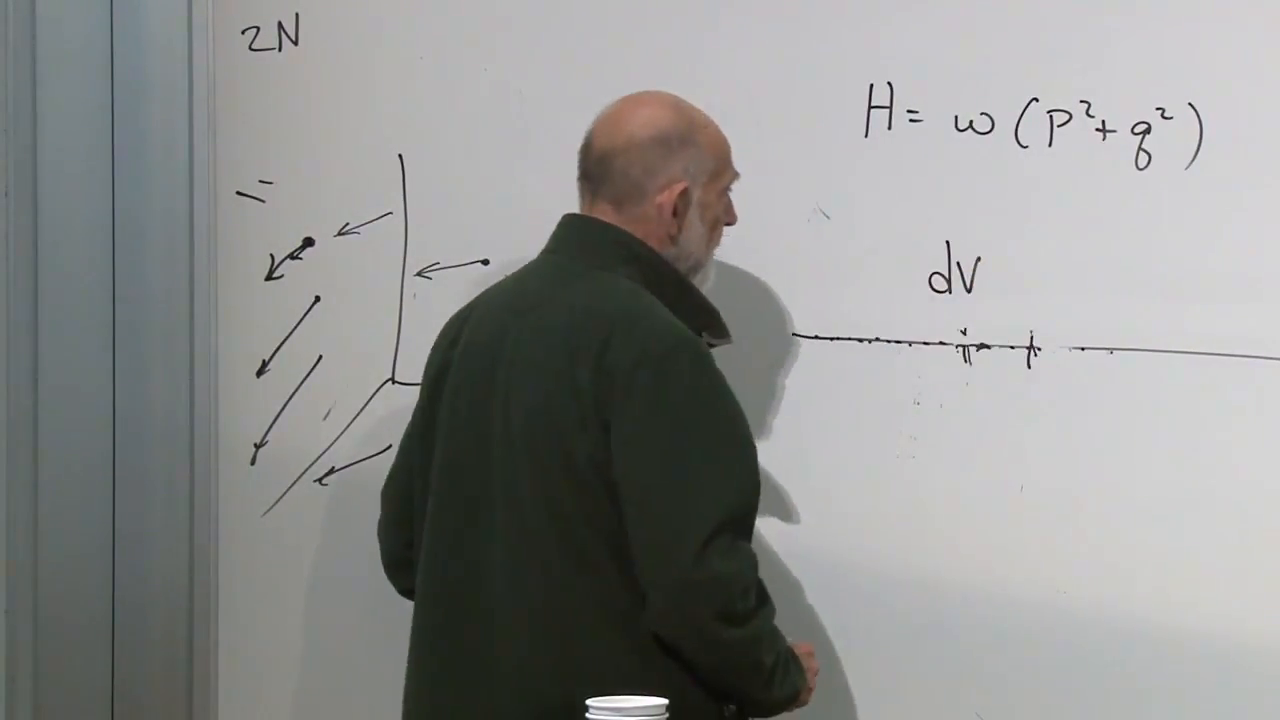
\includegraphics[width=0.84\textwidth]{lecture_07_figure_06.png}
  \caption{局所的な伸びまたは圧縮の割合としての\(dv/dx\)に至る一次元の構成。}
  \lectureframe{00:30:20}
\end{figure}

二つの等価な見方がある。物質的な区間を追い、その長さが変化するかを問うてもよい。あるいは小さな区間を固定し、単位時間あたりに入る量が去る量に等しいかを問うてもよい。前者は流体を追い、後者は流体が通り過ぎるのを見る。

一次元より多い場合、領域は一つの軸に沿って伸び、別の軸に沿って圧縮されても全体の体積は変化しないことがある。速度場\(\mathbf V=(V_x,V_y,V_z)\)に対して、関連する局所的な割合は発散であり、
\begin{equation}
  \nabla\cdot\mathbf V
  =
  \frac{\partial V_x}{\partial x}
  +\frac{\partial V_y}{\partial y}
  +\frac{\partial V_z}{\partial z}.
  \label{eq:l7-spatial-divergence}
\end{equation}
正の発散は局所的な膨張、負の発散は局所的な収縮であり、非圧縮性は
\begin{equation}
  \nabla\cdot\mathbf V=0.
  \label{eq:l7-zero-divergence}
\end{equation}
である。固定した小さな箱を通る流入と流出が等しいことは、運動する小さな箱の体積が保たれることと同じ局所的な主張である。

\begin{figure}[htbp]
  \centering
  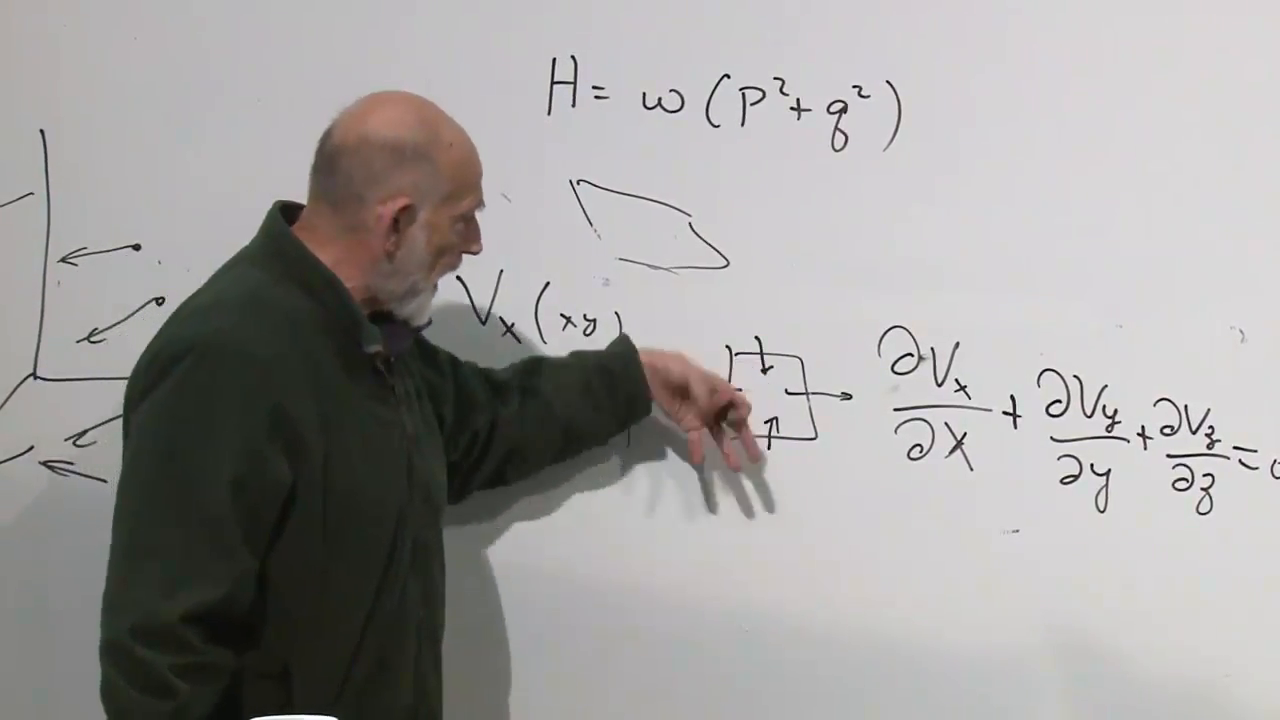
\includegraphics[width=0.86\textwidth]{lecture_07_figure_07.png}
  \caption{二次元の箱、その流れの成分、および発散を定義する同座標の導関数の和。}
  \lectureframe{00:35:30}
\end{figure}

\begin{classroomqa}
  \audiencequestion{我々は通常空間の流体について論じているのか、それとも位相空間の流れについて論じているのか。\lecturetimestamp{00:34:27--00:34:40}}
  \lecturerresponse{発散の議論はまず一般的な流体の議論である。それを偶数次元の位相空間に適用する。そこでは座標方向が\(q_i\)と\(p_i\)であり、速度成分が\(\dot q_i\)と\(\dot p_i\)である。}
\end{classroomqa}

ここで離散的な状態写像に戻る。可逆なサイクルでは、各ノードは一本の矢印が入り一本の矢印が出ており、選ばれた状態の集まりは時間発展しても同じ要素数を保つ。吸い込みでは、多くの矢印が入り、出るものは少なすぎる。いくつかの代替案は区別できなくなる。

\begin{figure}[htbp]
  \centering
  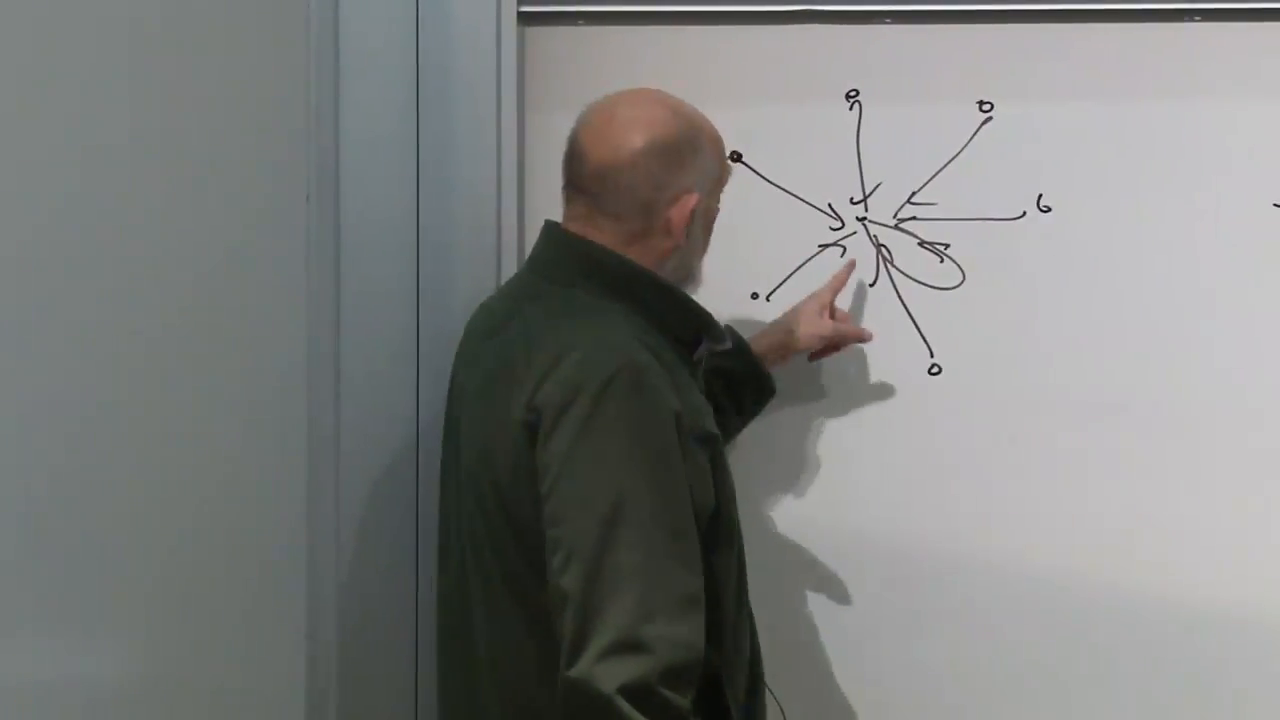
\includegraphics[width=0.80\textwidth]{lecture_07_figure_08.png}
  \caption{発散を第一講の可逆法則の判定法と再び結びつけるために用いられる離散的な吸い込み。}
  \lectureframe{00:40:15}
\end{figure}

連続的な問いは今や正確である。ハミルトン流は発散がゼロであり、したがって区別可能な状態の小さな領域がより小さな位相空間体積に押しつぶされることは決してないのか。

\section{リウヴィルの定理}

\begin{theorem}[Liouville's theorem]
滑らかなハミルトン系では、正準位相空間速度場の発散はゼロである。
\begin{equation}
  \sum_i\left(
    \frac{\partial\dot q_i}{\partial q_i}
    +\frac{\partial\dot p_i}{\partial p_i}
  \right)=0.
  \label{eq:l7-liouville-divergence}
\end{equation}
等価に、ハミルトン的時間発展は正準位相空間体積\(dq_1\cdots dq_n\,dp_1\cdots dp_n\)を保つ。
\end{theorem}

\begin{classroomqa}
  \audiencequestion{\(V\)と呼ばれる成分は単に\(p\)のドットと\(q\)のドットなのか。\lecturetimestamp{00:42:20--00:43:22}}
  \lecturerresponse{はい。一対については、
  \(V_q=\dot q\)および\(V_p=\dot p\)である。そのようなすべての導関数を並べると、全位相空間における流れの速度ベクトルが得られる。}
\end{classroomqa}

一つの正準対について、ハミルトンの方程式は
\begin{equation}
  V_p=-\frac{\partial H}{\partial q},
  \qquad
  V_q=\frac{\partial H}{\partial p}.
  \label{eq:l7-liouville-components}
\end{equation}
を与える。したがって発散は
\begin{align}
  \frac{\partial V_p}{\partial p}
  +\frac{\partial V_q}{\partial q}
  &=
  -\frac{\partial}{\partial p}
    \left(\frac{\partial H}{\partial q}\right)
  +\frac{\partial}{\partial q}
    \left(\frac{\partial H}{\partial p}\right)\\
  &=
  -\frac{\partial^2H}{\partial p\,\partial q}
  +\frac{\partial^2H}{\partial q\,\partial p}
  =0.
  \label{eq:l7-liouville-proof}
\end{align}

\begin{figure}[htbp]
  \centering
  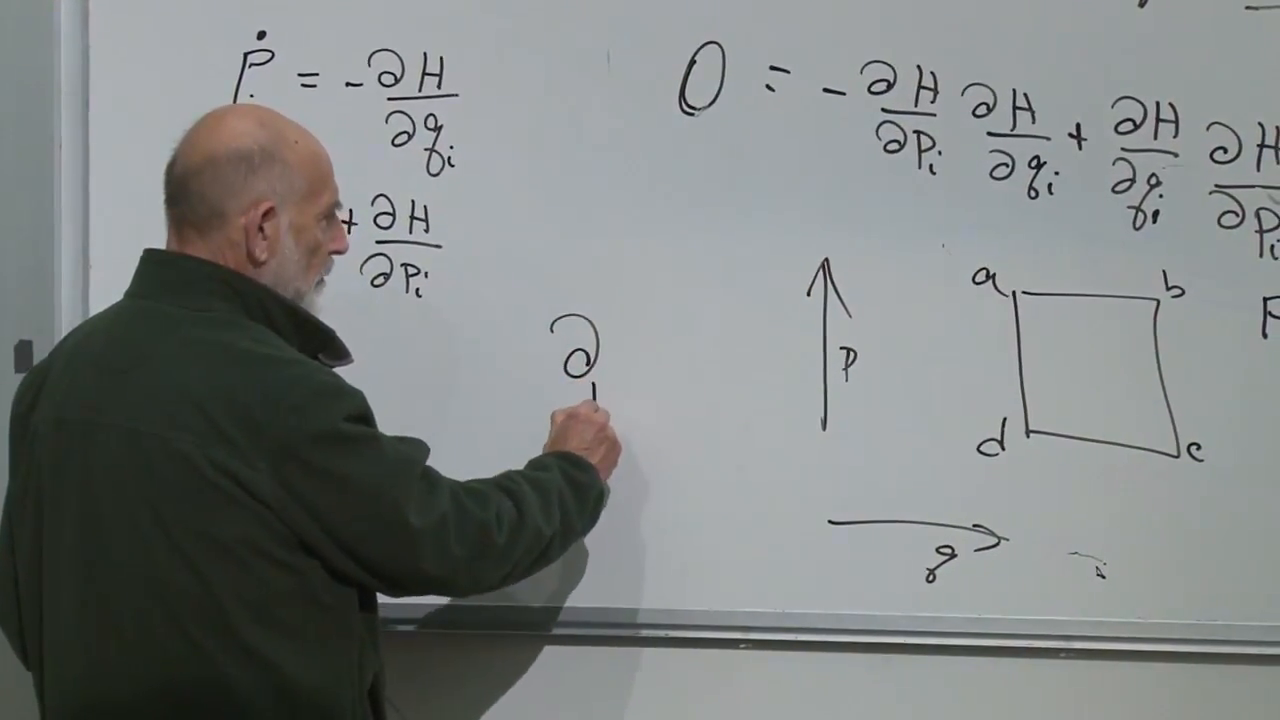
\includegraphics[width=0.86\textwidth]{lecture_07_figure_09.png}
  \caption{滑らかな混合偏導関数が可換である理由を説明するために用いられる有限差分長方形。}
  \lectureframe{00:47:30}
\end{figure}

混合偏導関数の等しさは、\(q\)-\(p\) 平面内の小さな長方形の四隅にある近接した4点 \(A,B,C,D\) によって理解できる。まず \(q\)-差分を取り、次に \(p\)-差分を取ると、2つの小さな辺の長さを除いて
\begin{equation}
  F(B)+F(D)-F(A)-F(C).
  \label{eq:l7-finite-difference-combination}
\end{equation}
が得られる。逆の順序で差分を取っても同じ組み合わせが得られる。小長方形の極限では、必要な導関数が連続であるならば、これは
\(\partial_p\partial_qF=\partial_q\partial_pF\)
である。

\begin{figure}[htbp]
  \centering
  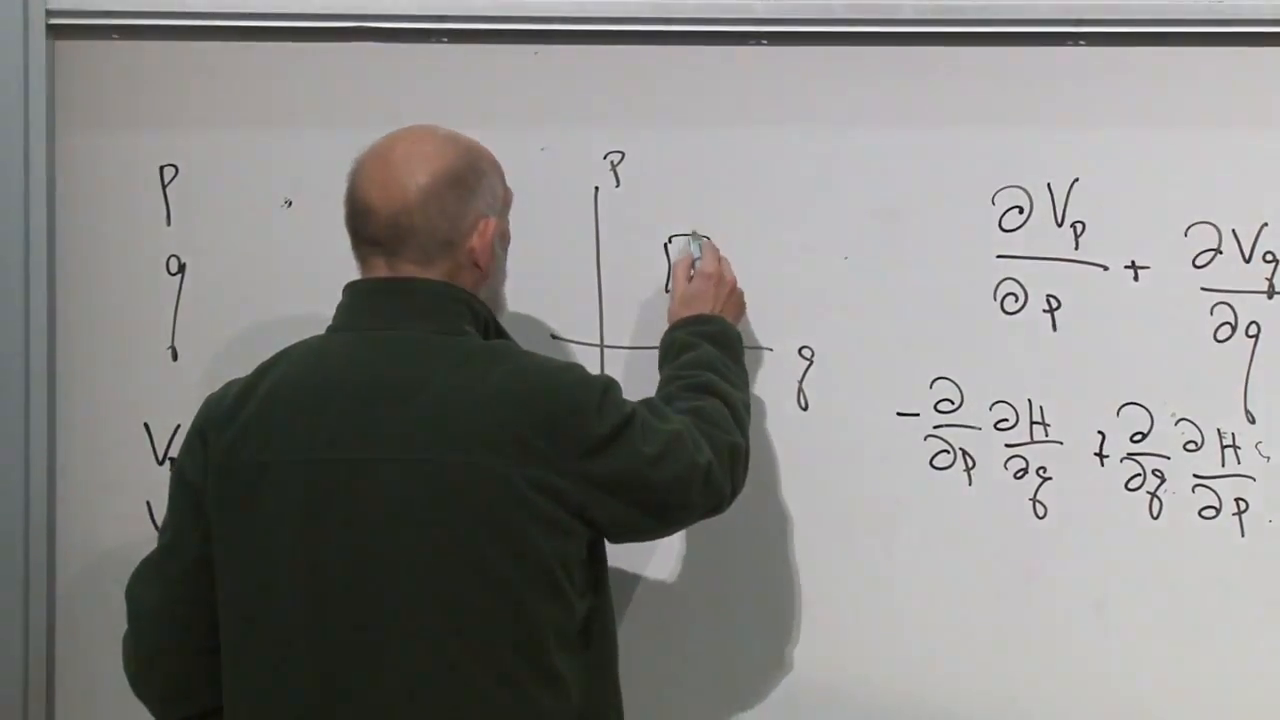
\includegraphics[width=0.88\textwidth]{lecture_07_figure_10.png}
  \caption{ハミルトンの方程式がそれを反対符号の2つの混合導関数に還元した後の正準発散。}
  \lectureframe{00:50:20}
\end{figure}

多くの自由度に対して、同じ相殺が各正準対ごとに起こる：
\begin{align}
  \sum_i\left(
    \frac{\partial\dot p_i}{\partial p_i}
    +\frac{\partial\dot q_i}{\partial q_i}
  \right)
  &=
  \sum_i\left(
    -\frac{\partial^2H}{\partial p_i\,\partial q_i}
    +\frac{\partial^2H}{\partial q_i\,\partial p_i}
  \right)\\
  &=0.
  \label{eq:l7-many-pair-proof}
\end{align}
一方の正準方向への伸長は、その共役方向への圧縮によって釣り合う。この対ごとの相殺は、無関係な軸間の偶然の相殺よりも強い構造である。

\begin{classroomqa}
  \audiencequestion{すべての正準対にわたる和は理解されていますか？
  \lecturetimestamp{00:52:00--00:52:36}}
  \lecturerresponse{はい。式~\eqref{eq:l7-many-pair-proof}は
  \(i\)について和を取っており、2つの混合導関数は各
  \(q_i,p_i\)対の中で別々に相殺されます。}
\end{classroomqa}

\begin{classroomqa}
  \audiencequestion{表示された発散はデカルト座標に見えます。この定理は座標変換を経ても成り立ちますか？
  \lecturetimestamp{00:52:50--00:53:22,\allowbreak\ 00:58:18--00:58:40}}
  \lecturerresponse{自然な定式化は正準座標と正準体積要素
  \(dq_1\cdots dq_n\,dp_1\cdots dp_n\)を用いてなされます。正準変換、すなわちシンプレクティック変換は座標と運動量を同時に変化させ、その体積を保存します。任意の非正準座標では、ヤコビ因子が体積測度に含まれるべきであり、座標増分の素朴な積は不変である必要はありません。}
\end{classroomqa}

\begin{classroomqa}
  \audiencequestion{リウヴィルの定理は時間に依存しないハミルトニアンを必要としますか？\lecturetimestamp{00:53:43--00:55:51}}
  \lecturerresponse{いいえ。エネルギー保存は
  \(\partial H/\partial t=0\)を必要としましたが、発散の証明は固定された時間において
  \(q_i\)と\(p_i\)に関してのみ微分します。混合偏導関数は
  \(H(q,p,t)\)に対しても依然として相殺されます。したがって、時間に依存するハミルトニアンは、時間に依存するが瞬間的には体積を保存する正準流を生成します。}
\end{classroomqa}

\section{体積保存が意味することと意味しないこと}

初期条件の任意の小さな領域 \(R_0\) を取り、すべての点を時間 \(t\) の間発展させる。リウヴィルの定理によれば
\begin{equation}
  \operatorname{Vol}(R_t)=\operatorname{Vol}(R_0).
  \label{eq:l7-volume-preservation}
\end{equation}
領域は移動し、回転し、せん断され、長いフィラメントに伸びるかもしれない。保護されるのはその体積であり、形状ではない。有限の滑らかなハミルトン発展において、異なる相点が合体することはあり得ない。

有限時間に対して、滑らかなハミルトン流は、逆方向に発展させることによって得られる滑らかな逆写像を持つ可逆写像である。これはまた、連結した塊が切断されて非連結な部分になることはできないという教室での主張も説明する。流れは領域を連続的に変形させ、その位相を保存する。たとえ極端に細い首によって2つのローブが有限の解像度では分離して見えるとしてもである。

\begin{figure}[htbp]
  \centering
  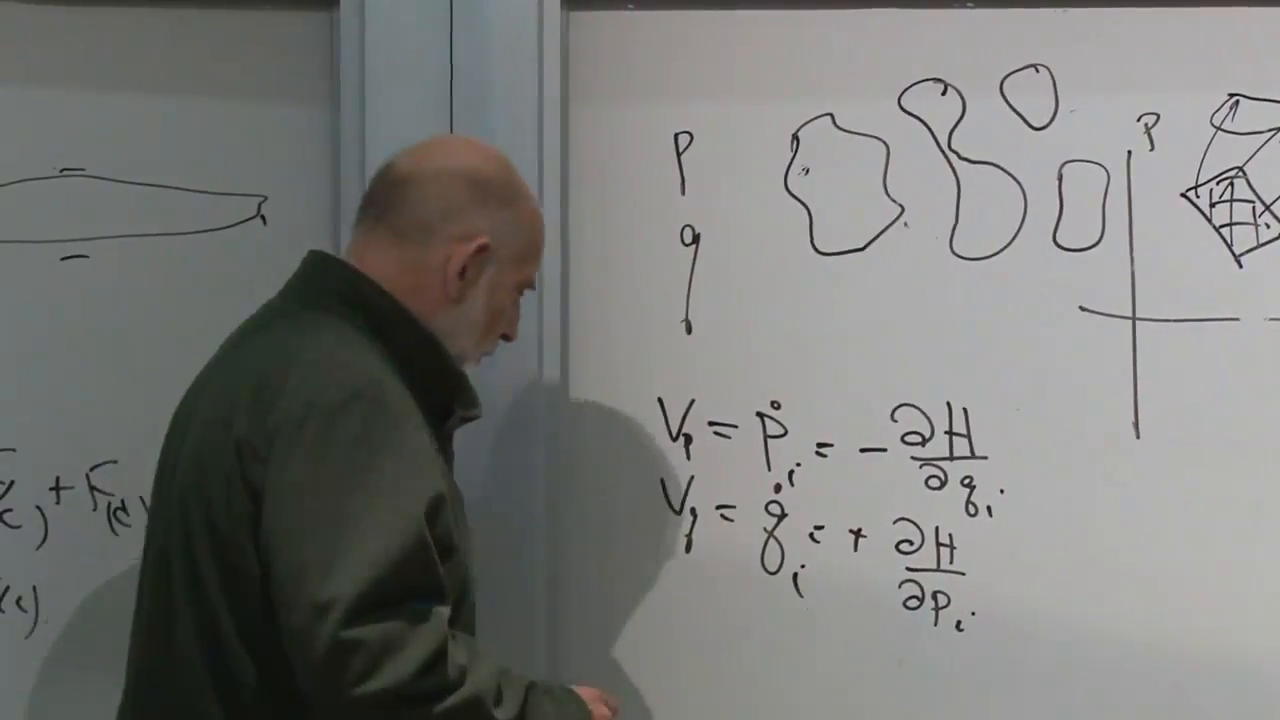
\includegraphics[width=0.86\textwidth]{lecture_07_figure_12.png}
  \caption{1つの相空間領域の可能な変形。滑らかなハミルトン流は細い首を生じさせ得るが、有限時間で独立に発展する部分への真の分裂は生じさせない。}
  \lectureframe{01:04:55}
\end{figure}

\begin{classroomqa}
  \audiencequestion{相空間領域はピンチオフして2つの部分に分裂できますか？\lecturetimestamp{01:04:10--01:05:49}}
  \lecturerresponse{有限時間の滑らかな決定論的ハミルトン流の下では分裂しない。仮想的なピンチ点においても、依然として1つの相空間点と1つの割り当てられた速度が存在し、2つの両立しない方向が存在するわけではない。領域は非常に長く狭い連結フィラメントを発達させ得るが、発展は一対一のままであり、それを引き裂くことはない。}
\end{classroomqa}

\begin{classroomqa}
  \audiencequestion{引き伸ばされた塊の広く離れた2つのローブは物理的に連結しているのか、それとも量子もつれしているのか？
  \lecturetimestamp{01:08:01--01:09:16}}
  \lecturerresponse{そのような物理的連結は含意されない。塊は代替的な初期条件の集合であり、1つの物質的対象ではない。それを1つの領域と呼ぶことは、それらの状態が発展してきた共通の集合を記録するものであり、それらの間の力や量子もつれについては何も述べていない。}
\end{classroomqa}

\begin{classroomqa}
  \audiencequestion{剛体振り子の直立した不安定平衡の近くでは何が起こるか。時計回りと反時計回りの軌道は重なり合うか。
  \lecturetimestamp{01:07:07--01:07:47}}
  \lecturerresponse{近傍の初期条件は、非常に異なる軌道へと分離し、先に述べた細いフィラメントを生じうる。それらが同一の相点になるのではない。微小変位または運動量の符号が両側を区別する。厳密に釣り合った状態は、それ自身の一意に定まる運動、すなわち理想模型において平衡にとどまるという運動をもつ。}
\end{classroomqa}

\subsection{位置空間における膨張と運動量空間における収縮}

正準変換が位置の範囲を因子\(a\)だけ膨張させるなら、共役な運動量のスケールは逆数の因子だけ収縮する：
\begin{equation}
  q\longrightarrow aq,
  \qquad
  p\longrightarrow \frac{p}{a},
  \qquad
  dq\,dp\longrightarrow dq\,dp.
  \label{eq:l7-canonical-scaling}
\end{equation}
これが気体膨張の例の背後にある明快な相空間の内容である。断熱膨張では、アクセス可能な通常空間の領域が成長する一方で、典型的な運動量は減少し、気体は冷却する。詳細な熱力学的関係は次元、膨張の手順、相互作用に依存する。リウヴィルの定理が与えるのは体積の制約であり、すべての熱力学的係数ではない。

\begin{classroomqa}
  \audiencequestion{同じ推論は膨張する宇宙にも当てはまるか、突然の膨張に対しても。\lecturetimestamp{00:53:23--00:56:00}}
  \lecturerresponse{リウヴィルの定理は、完全な力学がハミルトン的であるときはいつでも、陽に時間に依存する正準変数を含めて当てはまる。位置方向における膨張には、正準運動量方向における対応する収縮が伴わなければならない。しかしながら、宇宙論的スケール因子、気体の制御された膨張、自由に爆発する雲は同じ物理過程ではない。距離と後退速度の間のハッブル的な相関は、より速い物体がより遠くへ進むために生じうるのに対し、断熱冷却は局所的な運動量分布の収縮に関わる。いずれの場合も定理は完全な相空間写像を制約する。}
\end{classroomqa}

\begin{classroomqa}
  \audiencequestion{リウヴィルの定理にはどのような実用的な用途があるか。
  \lecturetimestamp{01:06:16--01:07:04}}
  \lecturerresponse{それは統計力学の中心である。微視的状態のアンサンブルがどのように発展するかを支配し、相空間体積とエントロピーの関係の基礎をなす。気体の膨張と冷却は一つの直接的な例示であり、後に平衡および非平衡の推論のための基本的な道具となる。}
\end{classroomqa}

\section{形を激しく変える流れ}

調和振動子はその流れが剛体回転であるため、面積と形の両方を保つ。それは例外的である。体積保存を剛性から分離するために、
\begin{equation}
  H=\lambda pq,
  \label{eq:l7-pq-hamiltonian}
\end{equation}
をとる。ここで\(\lambda\)は逆時間の単位をもつ。講義では\(\lambda=1\)と置く。それを保持すれば次元が明示的になる。

\begin{figure}[htbp]
  \centering
  \includegraphics[width=0.82\textwidth]{lecture_07_figure_03.png}
  \caption{\(H=pq\)の例の始まりと最初の相空間速度成分。}
  \lectureframe{01:00:11}
\end{figure}

ハミルトンの方程式は
\begin{equation}
  \dot p=-\lambda p,
  \qquad
  \dot q=\lambda q,
  \label{eq:l7-pq-flow}
\end{equation}
であり、解は
\begin{equation}
  p(t)=p_0e^{-\lambda t},
  \qquad
  q(t)=q_0e^{\lambda t}.
  \label{eq:l7-pq-solutions}
\end{equation}
である。正方形のパッチは\(p\)において指数的に圧縮され、\(q\)において同じ因子だけ引き伸ばされる：
\begin{equation}
  \Delta p(t)\Delta q(t)
  =
  \Delta p(0)\Delta q(0).
  \label{eq:l7-pq-area}
\end{equation}
その発散は結果を局所的に検証する、
\begin{equation}
  \frac{\partial\dot p}{\partial p}
  +\frac{\partial\dot q}{\partial q}
  =-\lambda+\lambda=0.
  \label{eq:l7-pq-divergence}
\end{equation}

\begin{figure}[htbp]
  \centering
  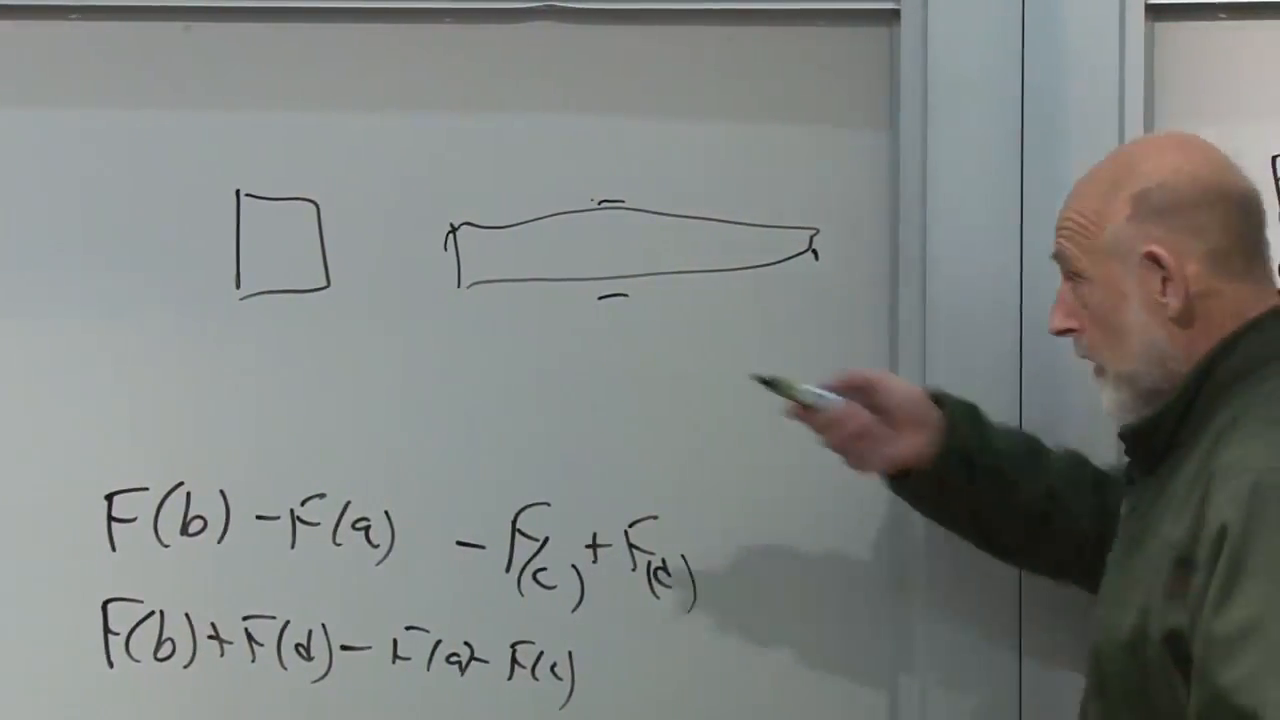
\includegraphics[width=0.86\textwidth]{lecture_07_figure_11.png}
  \caption{\(H=pq\)の流れの下で面積を保ちながら長く薄い帯へと引き伸ばされたコンパクトなパッチ。}
  \lectureframe{01:02:10}
\end{figure}

\begin{classroomqa}
  \audiencequestion{\(pq\)は作用の単位をもつので、リウヴィルの定理は作用の保存か。\lecturetimestamp{01:03:00--01:04:09}}
  \lecturerresponse{いいえ。定理は相空間体積を保存する。一つの正準対において、\(dq\,dp\)は作用の単位をもち、その次元的な事実は量子力学を予示する。そこでは相空間のセルが\(\hbar\)によって定まる単位で測られる。しかし積\(pq\)はそれ自体がハミルトンの作用汎関数ではなく、次元が一致するというだけで自動的に角運動量でもない。}
\end{classroomqa}

この例はまた、角度が保存される必要がないことを示す。式~\eqref{eq:l7-pq-solutions}のスケーリングの下で等しくない成分をもつ直角の十字は、その計量的な見かけにおいてずらされる一方、面積は変わらない。リウヴィルの定理は面積または体積の定理であり、通常のユークリッド的な剛性の定理ではない。

\section{減衰はシンクを生む}

定理が何を排除するかを見るために、減衰振動子の縮約された方程式を考える、
\begin{equation}
  m\ddot x=-kx-c\dot x,
  \qquad c>0.
  \label{eq:l7-damped-newton}
\end{equation}
\(p=m\dot x\)と置く。すると
\begin{equation}
  \dot x=\frac{p}{m},
  \qquad
  \dot p=-kx-\frac{c}{m}p.
  \label{eq:l7-damped-first-order}
\end{equation}
減衰がなければ、相点は原点の周りを回る。減衰があれば、エネルギーは周囲の媒質の微視的自由度へと移され、軌道は内向きに螺旋を描く。

\begin{figure}[htbp]
  \centering
  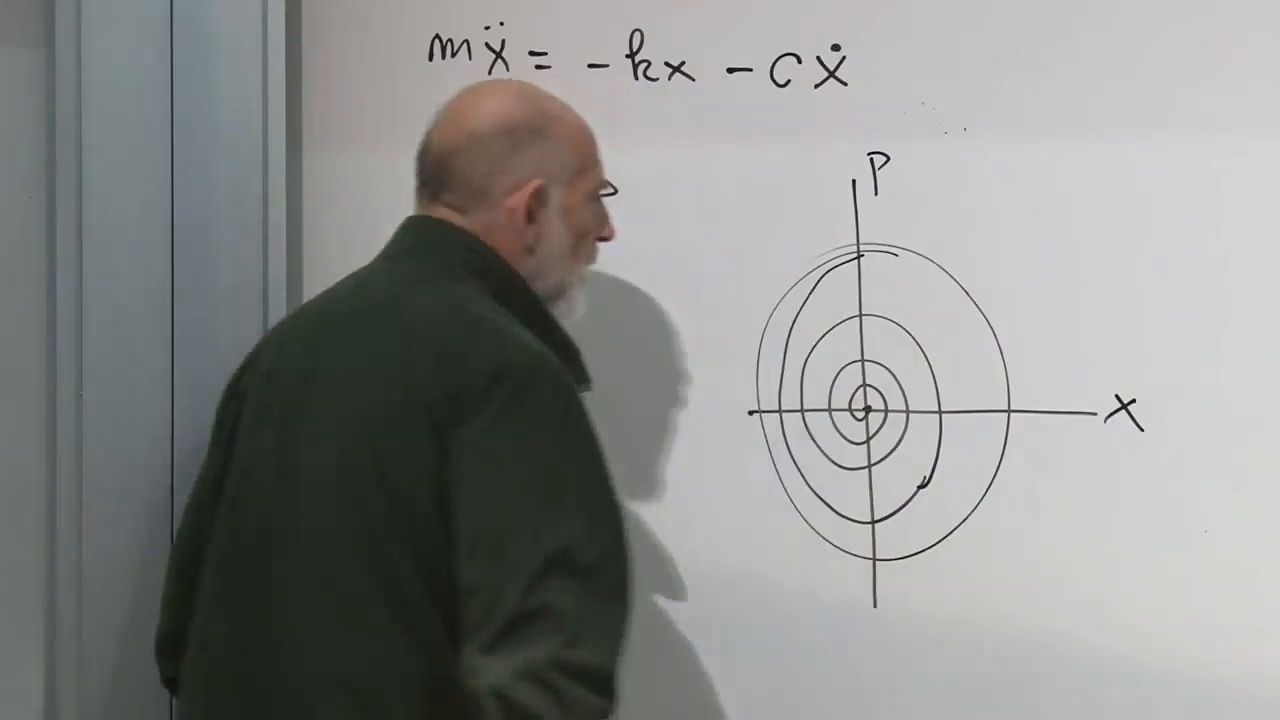
\includegraphics[width=0.84\textwidth]{lecture_07_figure_13.png}
  \caption{減衰振動子の方程式と\(x\)-\(p\)平面におけるその内向きの螺旋。}
  \lectureframe{01:13:30}
\end{figure}

この縮約された二次元の流れの発散は
\begin{equation}
  \frac{\partial\dot x}{\partial x}
  +\frac{\partial\dot p}{\partial p}
  =
  0-\frac{c}{m}<0.
  \label{eq:l7-damped-divergence}
\end{equation}
である。任意の有限な領域は収縮する。原点は吸い込みであり、多数の矢印が内向きの状態写像の連続版である。

\begin{figure}[htbp]
  \centering
  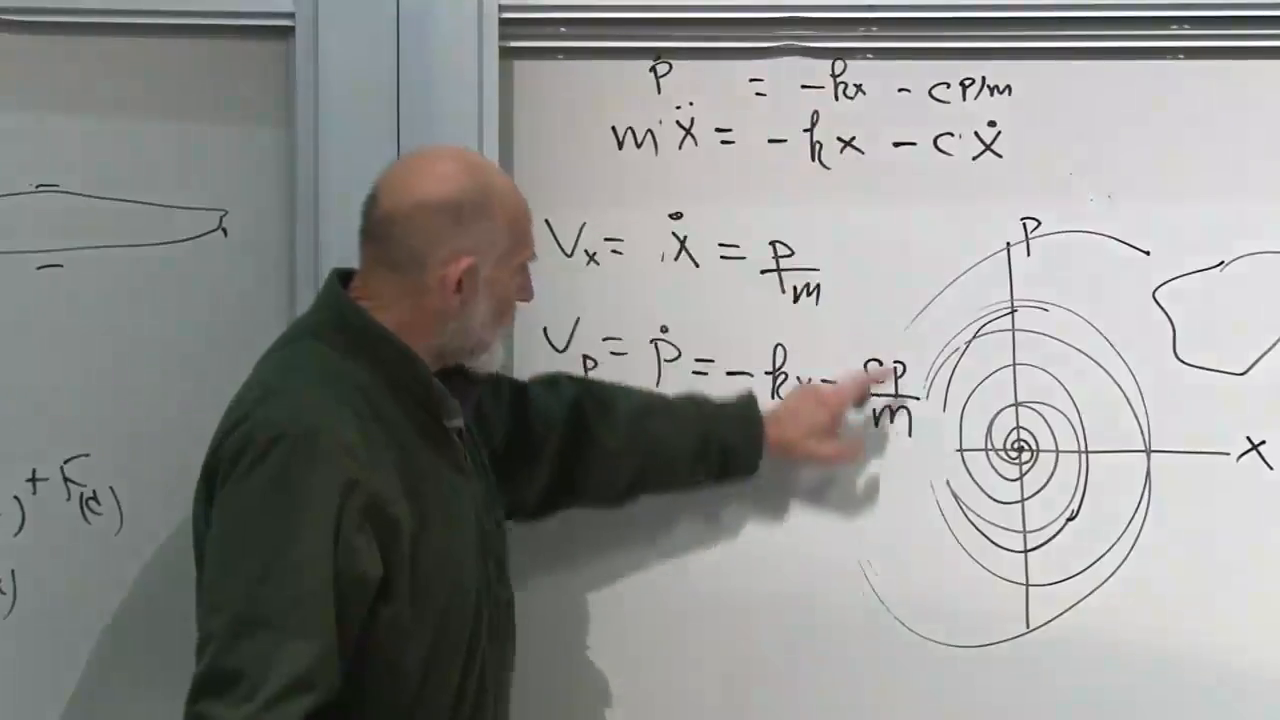
\includegraphics[width=0.88\textwidth]{lecture_07_figure_14.png}
  \caption{負の発散 \(-c/m\) を得るために用いた減衰位相空間速度成分。}
  \lectureframe{01:16:05}
\end{figure}

これは、微視的力学がリウヴィルの定理に反するという意味ではない。二つの変数 \(x,p\) は、振動子のエネルギーを受け取る膨大な数の環境自由度を省略している。拡大された振動子＋環境系は、その縮約された \(x,p\) 記述が収縮するとしても、ハミルトン的で体積保存的であり得る。

\begin{classroomqa}
  \audiencequestion{減衰振動子は、この縮約位相空間においてハミルトン的でないとしても、依然としてニュートンの方程式で記述されるのか。
  \lecturetimestamp{01:20:09--01:21:12}}
  \lecturerresponse{はい。ニュートンの \(F=ma\) は経験的に与えられた抗力項を含むことができる。初等的な \(L=T-V\) およびハミルトン的記述は保存力に直接適用され、より一般的なラグランジアンは速度に依存する力の一部も扱う。しかし、孤立した対 \(x,p\) に対するマルコフ的摩擦項は、閉じた正準ハミルトン系ではなく、縮約された散逸力学である。}
\end{classroomqa}

\begin{classroomqa}
  \audiencequestion{減衰方程式が無限精度で逆向きに積分できるなら、情報は本当に失われるのか。
  \lecturetimestamp{01:25:16--01:27:17}}
  \lecturerresponse{任意の有限時間に対して、理想的な微分方程式は依然として逆写像をもつので、厳密なデータを逆向きに走らせることができる。正確な言明は、有限の位相空間セルが指数関数的に収縮するということである。その過去を復元するには指数関数的に増大する精度が必要となり、無限時間ではすべての軌道が吸い込みに近づく。これは、離散的な選択肢の喪失像の最も近い連続古典的類似物であり、二つの厳密な有限時間解が文字通り一つになるという主張ではない。}
\end{classroomqa}

\begin{classroomqa}
  \audiencequestion{ベクトル場は、ハミルトン系に由来せずに発散がゼロになり得るか。\lecturetimestamp{01:18:21--01:22:34}}
  \lecturerresponse{もちろんである。ハミルトン形式は発散がゼロであるための十分条件であり、必要条件ではない。任意の非圧縮速度場は、同じ空間上の正準ハミルトン場でなくても発散がゼロになり得る。三次元非圧縮流体の速度場が教室での例である。三つの座標それ自体は正準対を形成できない。完全な流体力学はより洗練された無限次元ハミルトン形式をもつかもしれないが、それはここで述べている一方向の含意を逆にはしない。}
\end{classroomqa}

\section{問いによって明らかになるさらなる区別}

\begin{classroomqa}
  \audiencequestion{一定エネルギー面上の運動は、位相空間全体の体積の保存とどのように関係するのか。
  \lecturetimestamp{01:28:47--01:30:41}}
  \lecturerresponse{それらはハミルトン構造の独立な帰結である。\(H\) が時間に依存しなければ、各軌道はそれぞれ自身のエネルギー面上にとどまる。有限な領域はそのような面を多数横切ることがあり、リウヴィルの定理はその領域全体の体積が保存されると述べる。調和振動子では、流れが剛体回転であるため、領域はその形も保つ。\(H=pq\) の領域は面積のみを保ち、形は保たない。}
\end{classroomqa}

\begin{classroomqa}
  \audiencequestion{力学的仕事はハミルトン的説明のどこに位置づけられるのか。\lecturetimestamp{01:30:44--01:32:57}}
  \lecturerresponse{仕事は、選ばれた系の境界を越えて移動するエネルギーを記述する。外部の作用主体はおもりを持ち上げたりパラメータを変えたりして、それにより部分系のエネルギーを変えることができる。それが供給するエネルギーは作用主体から失われる。両側を一つの閉じたモデルに含めれば、重点は全エネルギー保存と部分系間の交換に戻る。}
\end{classroomqa}

\begin{classroomqa}
  \audiencequestion{体積保存は位相幾何学と角度も保存するのか。\lecturetimestamp{01:33:00--01:33:37}}
  \lecturerresponse{滑らかな有限時間ハミルトン流は、可逆な連続変形であるため位相幾何学を保存する。一般にはユークリッド的角度や形を保存しない。振動子の剛体回転はそれらを保存するが、\(H=pq\) の伸張は、それが特別な場合である理由を示している。}
\end{classroomqa}

\begin{classroomqa}
  \audiencequestion{ルジャンドル変換は物理的意義がないために省略されたのか。\lecturetimestamp{01:33:43--01:34:48}}
  \lecturerresponse{いいえ。それは速度による記述を運動量による記述に交換し、写像が正則なときに \(H=\sum_i p_i\dot q_i-L\) を生み出す有用な変換である。この構成は、その正式名称が強調されなかったときでさえすでに繰り返し用いられてきた。詳細な一般理論は、現在の定理には単に必要ないのである。}
\end{classroomqa}

\section{ポアソン括弧：次の圧縮}

最後の数分は歴史的な主題に戻る。19世紀の力学は、一見異なる体系を結びつける簡潔な構造を繰り返し探し求めた---力学と幾何光学、粒子と光線、古典的軌道と波動的記述。ポアソン括弧もそのような構造の一つであり、量子力学において特に重要になる。

\(F(q,p)\)を相空間上の任意の関数とする。それは座標かもしれないし、運動量かもしれないし、積\(qp\)かもしれないし、角運動量かもしれない。運動に沿って、
\begin{equation}
  \frac{dF}{dt}
  =
  \sum_i\left(
    \frac{\partial F}{\partial q_i}\dot q_i
    +\frac{\partial F}{\partial p_i}\dot p_i
  \right).
  \label{eq:l7-f-time-derivative}
\end{equation}
ハミルトンの方程式を代入すると、
\begin{equation}
  \frac{dF}{dt}
  =
  \sum_i\left(
    \frac{\partial F}{\partial q_i}
    \frac{\partial H}{\partial p_i}
    -
    \frac{\partial F}{\partial p_i}
    \frac{\partial H}{\partial q_i}
  \right).
  \label{eq:l7-f-hamiltonian-derivative}
\end{equation}

\begin{figure}[htbp]
  \centering
  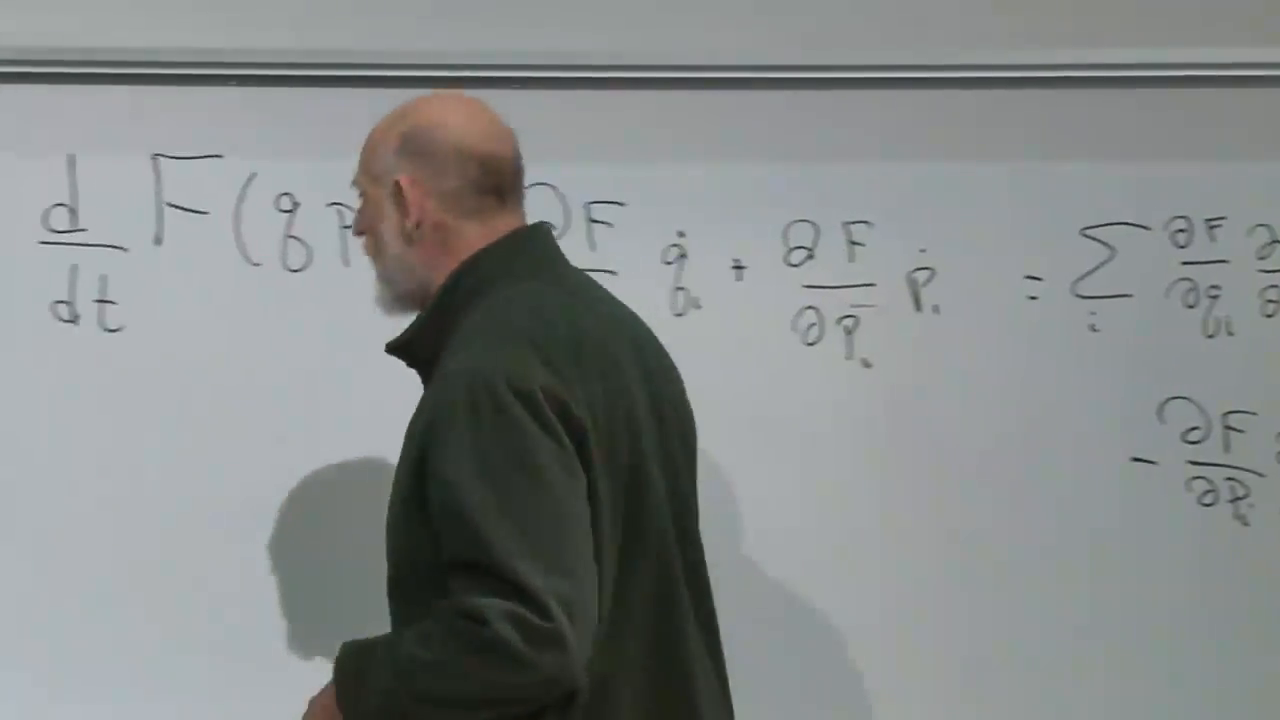
\includegraphics[width=0.88\textwidth]{lecture_07_figure_15.png}
  \caption{一般の相空間関数\(F(q,p)\)の時間微分に対する連鎖律。}
  \lectureframe{01:42:40}
\end{figure}

この繰り返し現れる反対称な組み合わせには名前がふさわしい。任意の二つの関数\(F\)と\(G\)に対し、それらのポアソン括弧を次で定義する：
\begin{equation}
  \boxed{
  \{F,G\}
  =
  \sum_i\left(
    \frac{\partial F}{\partial q_i}
    \frac{\partial G}{\partial p_i}
    -
    \frac{\partial F}{\partial p_i}
    \frac{\partial G}{\partial q_i}
  \right).}
  \label{eq:l7-poisson-bracket}
\end{equation}

\begin{figure}[htbp]
  \centering
  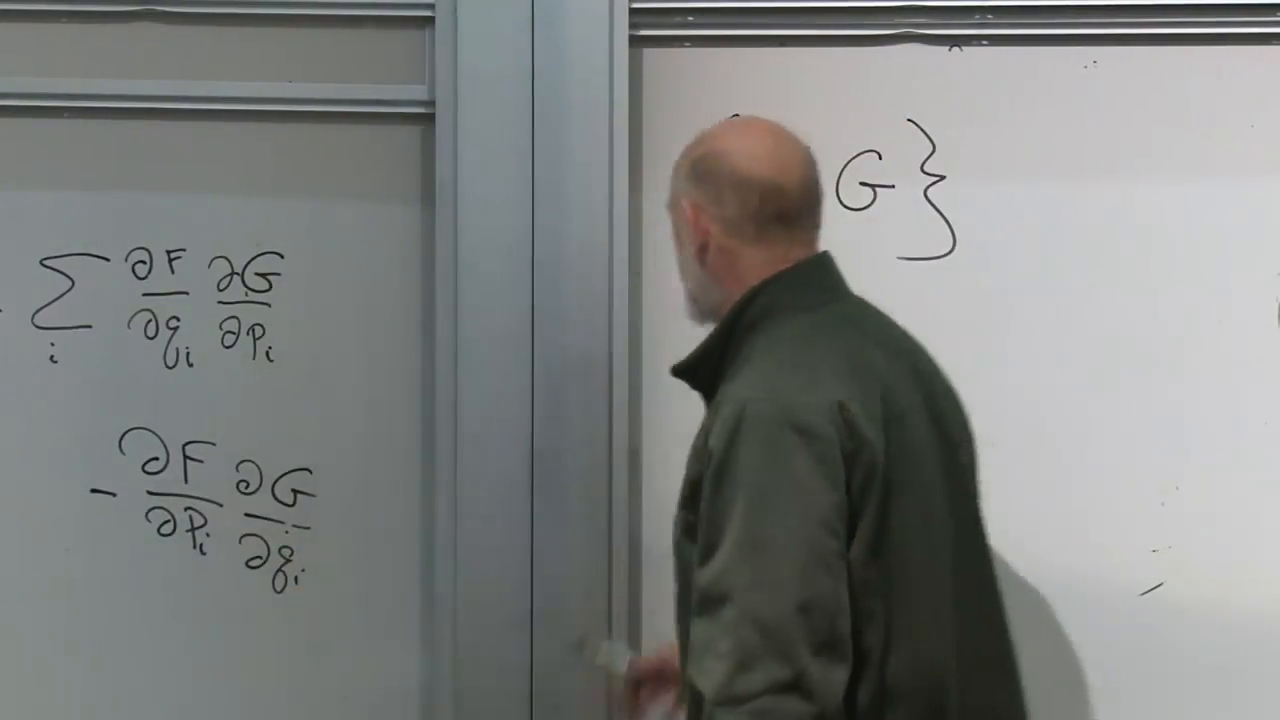
\includegraphics[width=0.86\textwidth]{lecture_07_figure_16.png}
  \caption{二関数の微分の組み合わせがポアソン括弧へと昇格したもの。}
  \lectureframe{01:44:15}
\end{figure}

式~\eqref{eq:l7-f-hamiltonian-derivative}は次のようになる：
\begin{equation}
  \boxed{\frac{dF}{dt}=\{F,H\}.}
  \label{eq:l7-hamiltonian-poisson-evolution}
\end{equation}
\(F\)がさらに陽に時間に依存するなら、\(\partial F/\partial t\)を加える。\(F=q_i\)または\(F=p_i\)と取るとハミルトンの二つの方程式が回復されるので、式~\eqref{eq:l7-hamiltonian-poisson-evolution}は完全な力学の簡潔な形である。

表記はいつでも人為的に圧縮できる---多くの方程式を二乗し、それらを足し合わせ、その結果を一つの方程式と呼ぶこともできよう。それは構造を明らかにするのではなく隠すであろう。ポアソン括弧が有用なのは逆の理由による。その代数が時間発展、保存量、対称性を組織するのである。次の段階はその代数を展開し、それを角運動量に用いることである。その構造は古典力学においても量子論においても中心的となるであろう。

\section{可逆性の連続的な意味}

ここで、その筋道を短縮せずに述べることができる。ハミルトンの方程式は、ハミルトニアンが陽に時間に依存しないとき\(H\)を保存するので、個々の軌道は等エネルギー超曲面上にとどまる。同じ方程式が相空間の各点に速度を割り当てる。その速度の発散は、混合偏導関数が対ごとに相殺するため消える。したがって、可能な状態の領域全体がその正準体積を保つ。

これが、一つの矢印が入り一つの矢印が出るという事柄の連続版である。形は変わりうるし、角度も変わりうるし、隣接する軌道は甚だしく離れうる。滑らかで閉じたハミルトニアンの記述において起こりえないのは、有限個の選択肢の集まりがより小さな相空間体積へと圧縮されることである。\(H=pq\)の流れは引き伸ばす自由を示し、縮約された減衰振動子はハミルトニアンの条件が放棄されると現れる吸い込み口を示す。そしてポアソン括弧は、同じ力学を、ハミルトニアンがすべての時間微分を生成するという命題へと凝縮する。
